\documentclass[tikz,border=3.14mm]{standalone}
\begin{document}
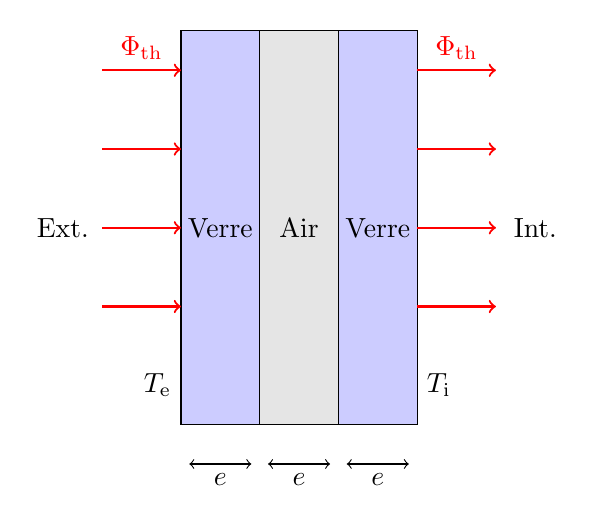
\begin{tikzpicture}

% Define the common length
\def\length{1}

% Glass panes
\draw[fill=blue!20] (0,0) rectangle (\length,5) node[midway] {Verre};
\draw[fill=blue!20] (2*\length,0) rectangle (3*\length,5) node[midway] {Verre};

% Air gap
\draw[fill=gray!20] (\length,0) rectangle (2*\length,5) node[midway] {Air};

% Width of glass and air gap
\draw[<->,shorten <=3pt, shorten >=3pt] (0,-0.5) -- (\length,-0.5) node[midway, below] {$e$};
\draw[<->,shorten <=3pt, shorten >=3pt] (\length,-0.5) -- (2*\length,-0.5) node[midway, below] {$e$};
\draw[<->,shorten <=3pt, shorten >=3pt] (2*\length,-0.5) -- (3*\length,-0.5) node[midway, below] {$e$};

% Arrows representing heat flow (from outside to inside)
\draw[->, red, thick] (-1,4.5) -- (0,4.5) node[above,midway] {$\Phi_{\rm th}$};
\draw[->, red, thick] (-1,3.5) -- (0,3.5);
\draw[->, red, thick] (-1,2.5) -- (0,2.5);
\draw[->, red, thick] (-1,1.5) -- (0,1.5);

% Labeling inside and outside
\node at (-1.5,2.5) {Ext.};
\node at (3*\length+1.5,2.5) {Int.};


% Temperature labels
\node[left] at (0,0.5) {$T_{\rm e}$};
\node[right] at (3*\length,0.5) {$T_{\rm i}$};

% Reduced heat flow
\draw[->, red, thick] (3*\length,4.5) -- (3*\length+1,4.5) node[above,midway] {$\Phi_{\rm th}$};
\draw[->, red, thick] (3*\length,3.5) -- (3*\length+1,3.5);
\draw[->, red, thick] (3*\length,2.5) -- (3*\length+1,2.5);
\draw[->, red, thick] (3*\length,1.5) -- (3*\length+1,1.5);

% Heat transfer and insulation description
% \node at (1.6,-0.5) {Double Glazed Window (Improved Insulation)};
\end{tikzpicture}
\end{document}
